\documentclass[12pt,oneside,a4paper]{article}

\usepackage[backend=biber,style=numeric]{biblatex}
\usepackage{xcolor}
\usepackage{todonotes}
\usepackage{amsmath}
\usepackage{multicol}
\usepackage{caption}
\usepackage{hyperref}
\usepackage{graphicx}
\usepackage{listings}
\lstset{
	frame=top,frame=bottom,
	language=C,
	basicstyle=\small\normalfont,
	xleftmargin=\parindent,
	keywordstyle=\color{green!40!black},
	%  commentstyle=\itshape\color{purple!40!black},
	%  identifierstyle=\color{blue},
	%  stringstyle=\color{orange},
	morekeywords={in, globaldata, procedure, input, output, behavior, end, XOR, NOT, AND}, % keyword to highlight
	%  captionpos=t,
	tabsize=2,
	numbers=left,
	stepnumber=1,                   % the step between two line-numbers.        
	numbersep=5pt,
	framexleftmargin=10pt,
	title=\lstname,
	captionpos=t,
	showspaces=false,
}
\DeclareCaptionFormat{listing}{\rule{\dimexpr\textwidth\relax}{0.4pt}\par\vskip1pt#1#2#3}
\captionsetup[lstlisting]{format=listing,singlelinecheck=false, margin=0pt,labelsep=space,labelfont=bf}

\usepackage{booktabs}
\usepackage[noabbrev,capitalise]{cleveref}
\crefname{listing}{algorithm}{algorithms}
\Crefname{listing}{Algorithm}{Algorithms}
\renewcommand\lstlistingname{Algorithm}
\def\lstlistingcrefname{Algorithm}
\usepackage{url}

\addbibresource{biblio.bib}

\title{\textbf{NecstCAMP \& CrossFit}}

\author{Manuel Colombo}

\date{2023}

\begin{document}


\begin{titlepage}
	\centering
	\clearpage
	\maketitle
	\thispagestyle{empty}
	\vspace*{1cm}
	\vfill
	\centering
	
\includegraphics{logo_polimi.png}
\includegraphics{logo_NECST.png}
\end{titlepage}


\section{Introduzione} \label{sec:intro}
La consapevolezza nel CrossFit è un elemento fondamentale per il successo nell'allenamento. Può essere paragonata al teorema del navigatore, in cui è importante sapere esattamente dove si desidera arrivare, ma ancor più cruciale è essere consapevoli di dove ci si trova attualmente (la propria consapevolezza). Conoscere i propri limiti e confini è essenziale per progredire, perché siamo stati creati per muoverci in modo efficiente e se non utilizziamo questa capacità, la perdiamo.. . L'obiettivo è migliorare i movimenti utili nella vita quotidiana, e l'allenamento nel CrossFit, caratterizzato da un'alta intensità, incoraggia a uscire dalla zona di comfort, poiché è proprio lì che si trova la crescita personale. Sono sufficienti solo 45 minuti di esercizio per migliorare l'intera giornata.  

\section{La gerarchia teorica dello sviluppo di un atleta} \label{sec:aleben}
La gerarchia teorica dello sviluppo di un atleta può essere migliorata come segue: 

La base della piramide delo sviluppo di un atleta è la nutrizione, che rappresenta il fondamento per il recupero e la cura del corpo. Senza una corretta alimentazione, gli atleti non possono massimizzare il loro potenziale. 

Al di sopra della nutrizione, si trova la resistenza metabolica, che si riferisce alla capacità cardiovascolare. È importante che gli atleti sviluppino una buona resistenza per sostenere sforzi prolungati durante la competizione. 

Successivamente, viene la ginnastica, che riguarda la capacità di muovere il corpo nello spazio. La flessibilità, l'equilibrio e la coordinazione sono elementi chiave della ginnastica e contribuiscono alla performance atletica. 

Un altro elemento cruciale è il sollevamento di carichi rispetto al proprio corpo. Questo tipo di allenamento aiuta a sviluppare la forza muscolare e la resistenza. Gli atleti devono essere in grado di sollevare pesi adeguati per supportare le esigenze specifiche del loro sport. 

All'interno di questa gerarchia teorica, le abilità specifiche dello sport si trovano in cima.
\newpage
\begin{figure}[h]
    \centering
    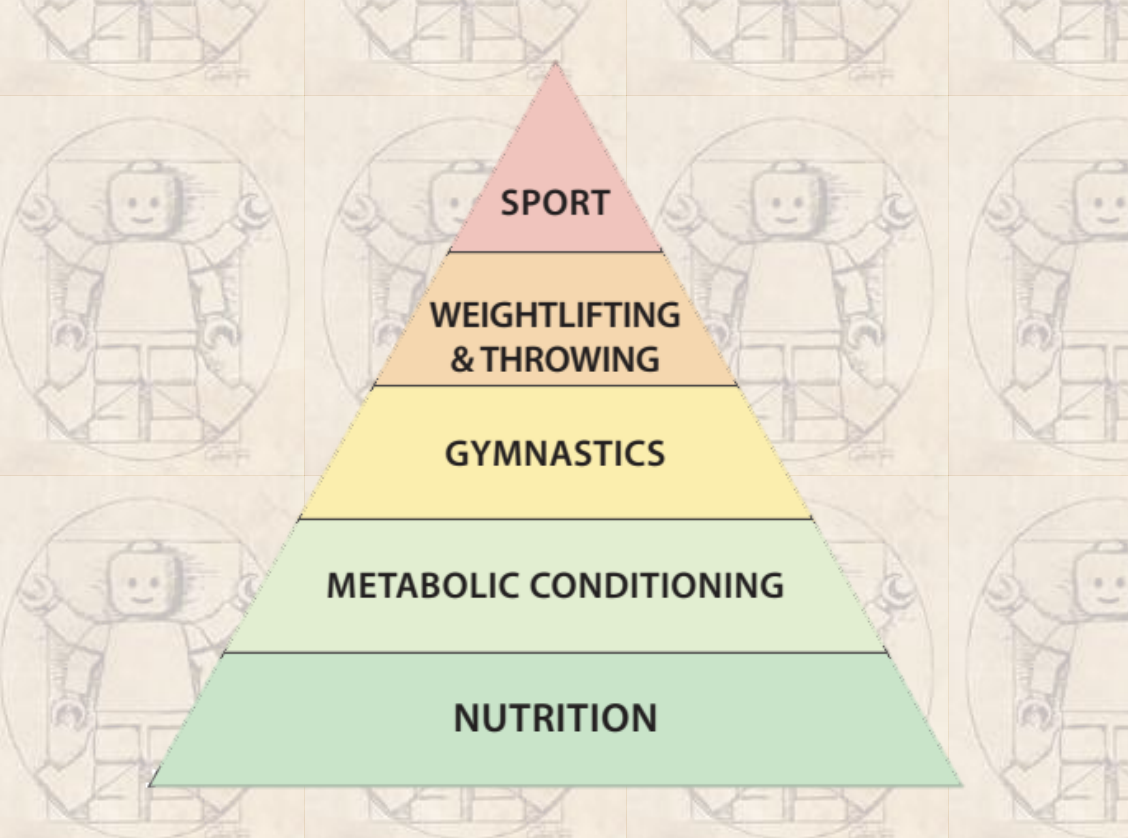
\includegraphics[width=.7\textwidth]{pircross.png}
    \caption{CrossFit Level1 TrainingGuide}
    \label{fig:my_label}
\end{figure}
Queste abilità rappresentano il punto più ottimale del continuum di malattia-benessere-fitness, in cui l'allenamento costante porta da uno stato di malattia a uno di benessere e infine a uno di fitness. Tuttavia, se si smette di allenarsi, si può tornare indietro lungo la stessa linea, compromettendo le abilità acquisite e la condizione fisica raggiunta. 
\begin{figure}[h]
    \centering
    
\includegraphics[width=.9\textwidth]{linea.png}
    \caption{The Sickness-Wellness-Fitness Continuum}
    \label{fig:my_label}
\end{figure}

\section{Espandere il Potenziale attraverso la preparazione mente e corpo: Il Flusso verso il Successo} \label{sec:famem}
La Preparazione Fisica Generale (General Physical Preparedness) è un concetto che può essere applicato a diversi sport per migliorare le prestazioni complessive degli atleti. Questo approccio si concentra sullo sviluppo di dieci abilità cruciali: resistenza, resistenza muscolare, forza, flessibilità, potenza, velocità, coordinazione, agilità, equilibrio e precisione. L'obiettivo principale è espandere la capacità in ognuna di queste, tenendo conto del fatto che sia il cuore che la mente, ossia la volontà, svolgono un ruolo fondamentale nel raggiungimento delle prestazioni ottimali nello sport. 
\begin{figure}[h]
    \centering
    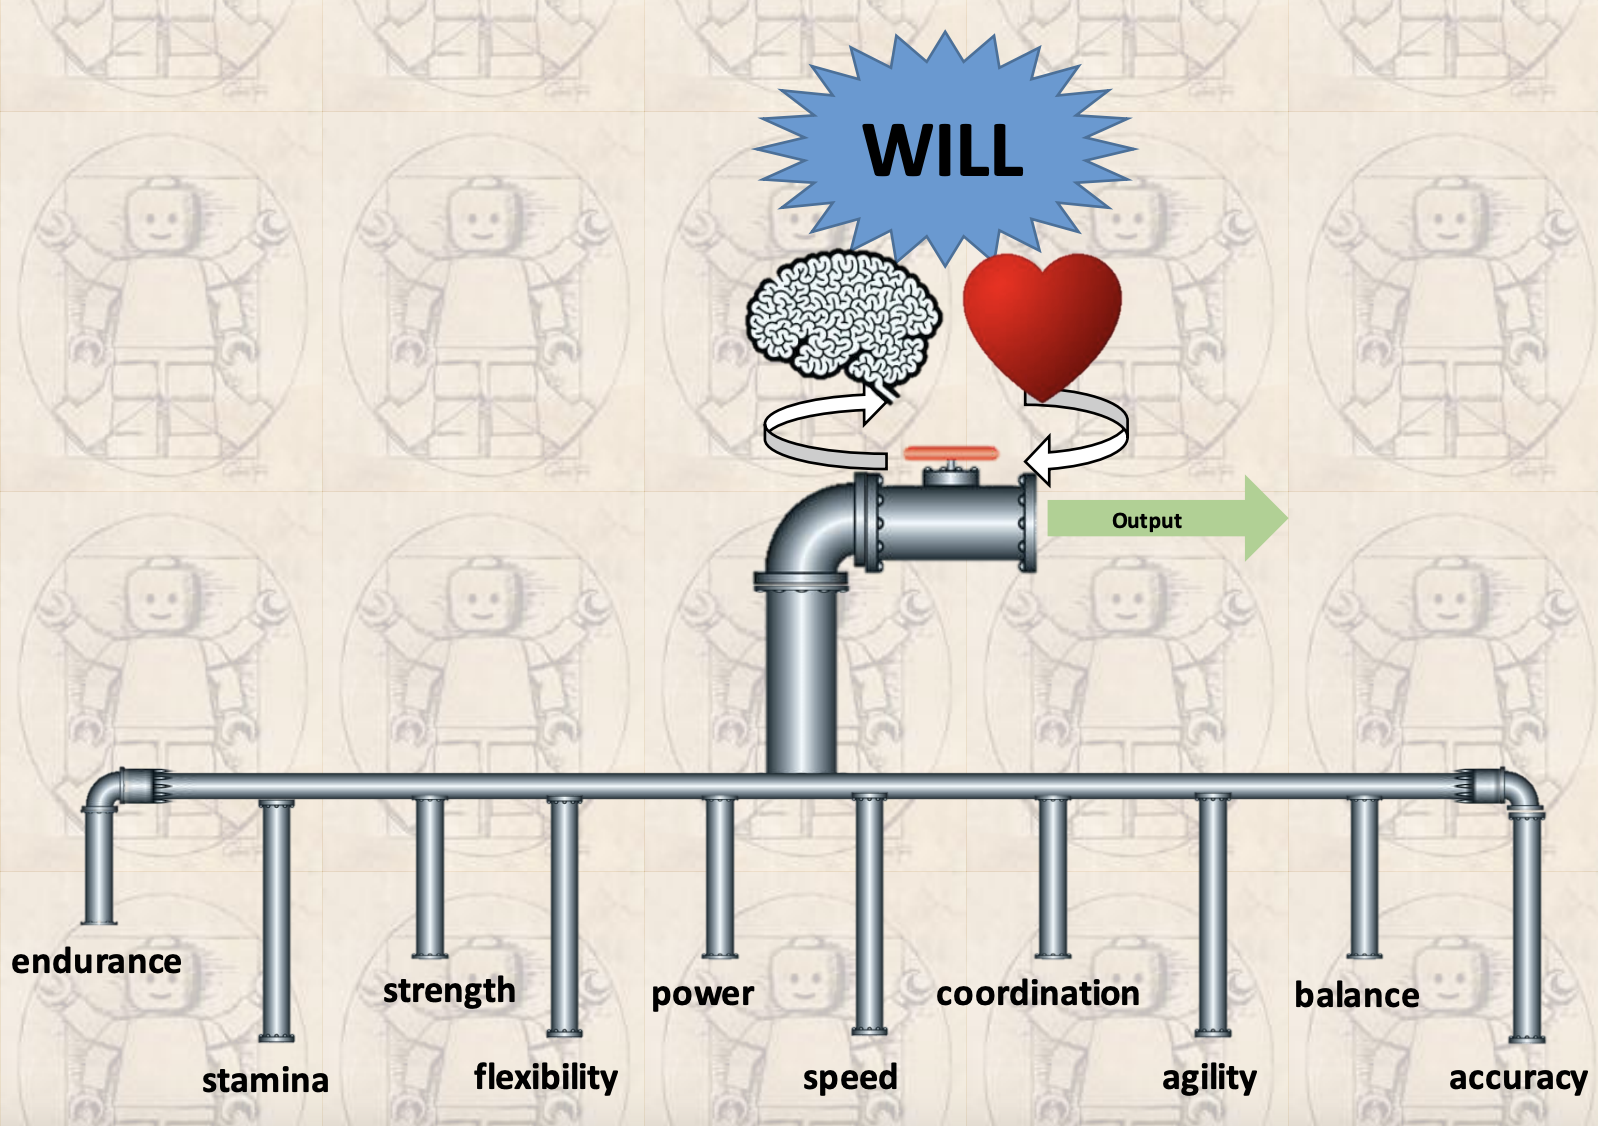
\includegraphics[width=.8\textwidth]{tubi.png}
    \label{fig:my_label}
\end{figure}

La chiave per sbloccare il proprio potenziale e raggiungere prestazioni ottimali nello sport è combinare l'approccio di Anders Ericsson, che vede il potenziale come un serbatoio espandibile, con l'implementazione della General Physical Preparedness. 

Secondo Anders Ericsson, il potenziale non è una scatola rigida e predefinita con cui si nasce, ma piuttosto un serbatoio espandibile che può essere sviluppato attraverso l'apprendimento. Ogni atleta può creare il proprio potenziale impegnandosi in sfide quotidiane, come ad esempio adottare una dieta equilibrata, seguire una corretta idratazione o eseguire gesti di gentilezza verso gli altri. L'obiettivo dovrebbe essere ambizioso, ma raggiungibile, in modo da spingere gli atleti a superare i propri limiti e migliorarsi costantemente. 
Nel caso di un fallimento, è importante non rimanere fermi solo a riflettere, ma agire senza farsi sopraffare dai pensieri negativi. Come affermava Samuel Beckett: "Hai fallito? Ricarica, ricalibra e continua ad andare avanti. Fallisci ancora, fallisci meglio." L'importante è perseverare e imparare dagli insuccessi al fine di progredire costantemente. Sono proprio le lezioni apprese attraverso i fallimenti che spingono gli atleti a migliorarsi e raggiungere nuovi livelli di successo nello sport. 
\begin{figure}[h]
    \centering
    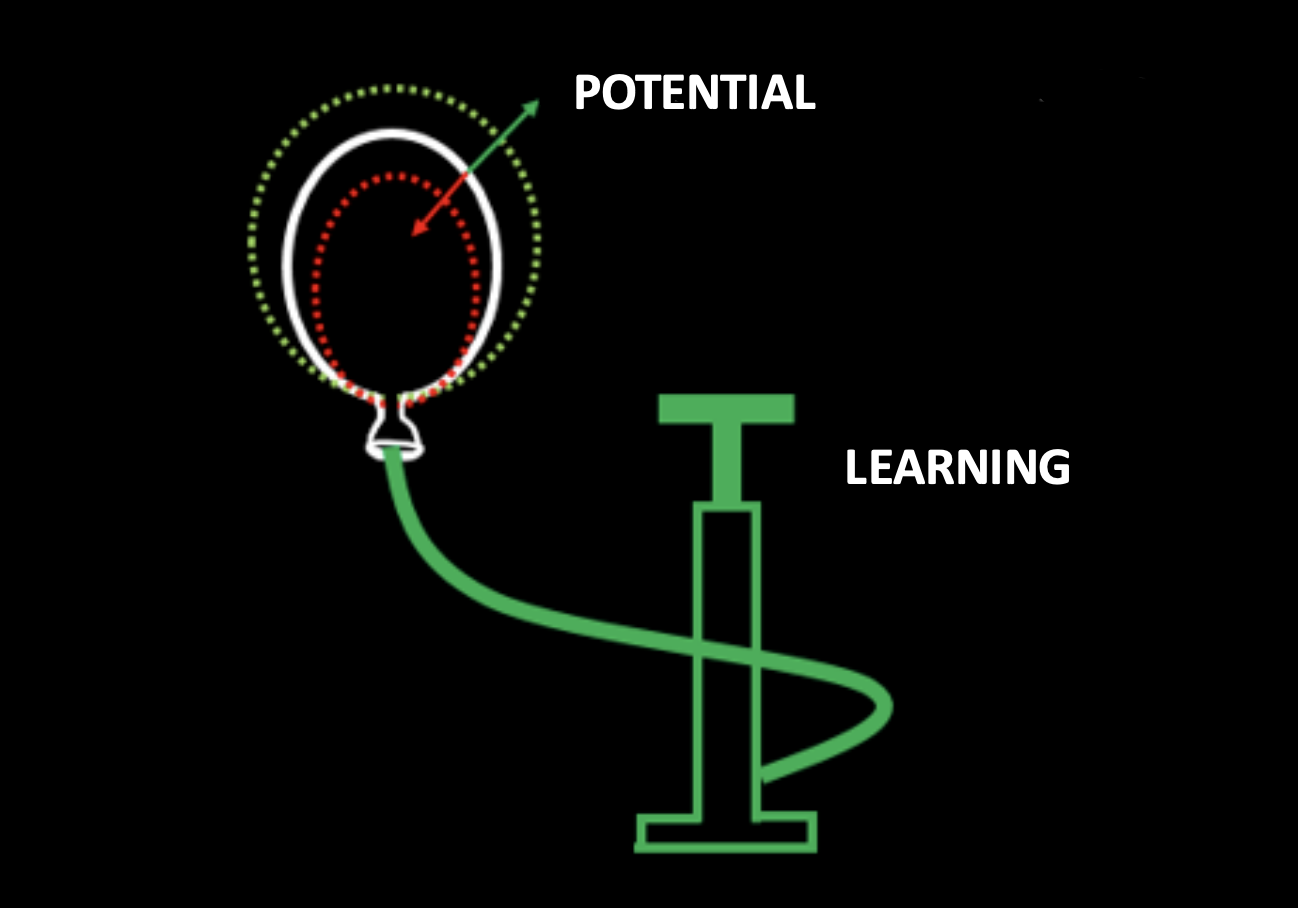
\includegraphics[width=.7\textwidth]{pall.png}
    \label{fig:my_label}
\end{figure}


\section{Conclusioni} \label{sec:concl}
In conclusione, una conoscenza approfondita di sé stessi, compresi i propri limiti e punti di forza, è essenziale per progredire in modo costante. Questa consapevolezza consente agli atleti di adattare le proprie strategie di allenamento in base alle proprie esigenze e di prendere decisioni durante le competizioni. 

Inoltre, l'allenamento ad alta intensità e la volontà di uscire dalla zona di comfort sono fattori comuni che stimolano la crescita e il miglioramento in tutti gli sport. 

Tuttavia, il successo nello sport non si basa solo sull'aspetto fisico, ma anche sull'aspetto mentale. Per sfruttare appieno il proprio potenziale, è necessario un approccio continuo di apprendimento che unisca la preparazione fisica generale con la determinazione di superare i propri limiti. Gli atleti devono essere pronti ad affrontare le sfide, imparare dalle esperienze passate e adattare le proprie strategie di allenamento di conseguenza. 

Infine, attraverso le lezioni apprese dai fallimenti, gli atleti possono raggiungere nuovi livelli di successo. Ogni fallimento è un'opportunità per crescere e imparare. 


\newpage
\title{\textbf{Bibliografia}} \\
\begin{itemize}
\item Meeting NecstCAMP del 04/10/2022 tenuto da Coach Andal
\item Meeting NecstCAMP del 25/03/2023 tenuto da Coach Andal
\end{itemize}

\end{document}


